\section{Sensor Description}

The sensor used in the experiment consists of a stereo pair of
cameras. Cameras are mounted on an XR4000 robot facing forward,
parallel to the ground plane. The two cameras were aligned to be
almost parallel to each other. The stereo base line is approximately 30
cm. The exact relative poses of the cameras were computed through
stereo calibration.

Internal camera parameters were determined by calibration for each of
the cameras. These cameras are capable of capturing colour images at a
maximum resolution of 640x480 at the rate of 30 frames per second,
however the image is obtained by interlacing. Camera captures odd rows
in one sweep and then even rows in the second sweep. These two halves
of the image, are called fields, and are transmitted one after
another. Each field is a 640x240 image. The complete image can then be
constructed by the capturing software from the two successive fields.
Since the two fields are captured at slightly different times, the
joined image might have undesired artefacts when the scene is not
static or when the robot is moving.

While the cameras can provide 30 frames per second, the computer on
the robot can successfully capture and store 15 fields from each
camera at most.  Sustainable throughput is even less at 11-12 fields
per seconds, due to the limitations of the recording system. Captured
frames are stored to the on-board hard drive as separate files.

The odd and even fields are very similar, so there is little extra
information to be gained from the second field. Faster frame rate is
more important, therefor only odd fields from both cameras are
recorded at a sustainable rate of 11.5 per second.

\begin{figure}[htbp]
  \centering
\subfigure[Original image.]{
  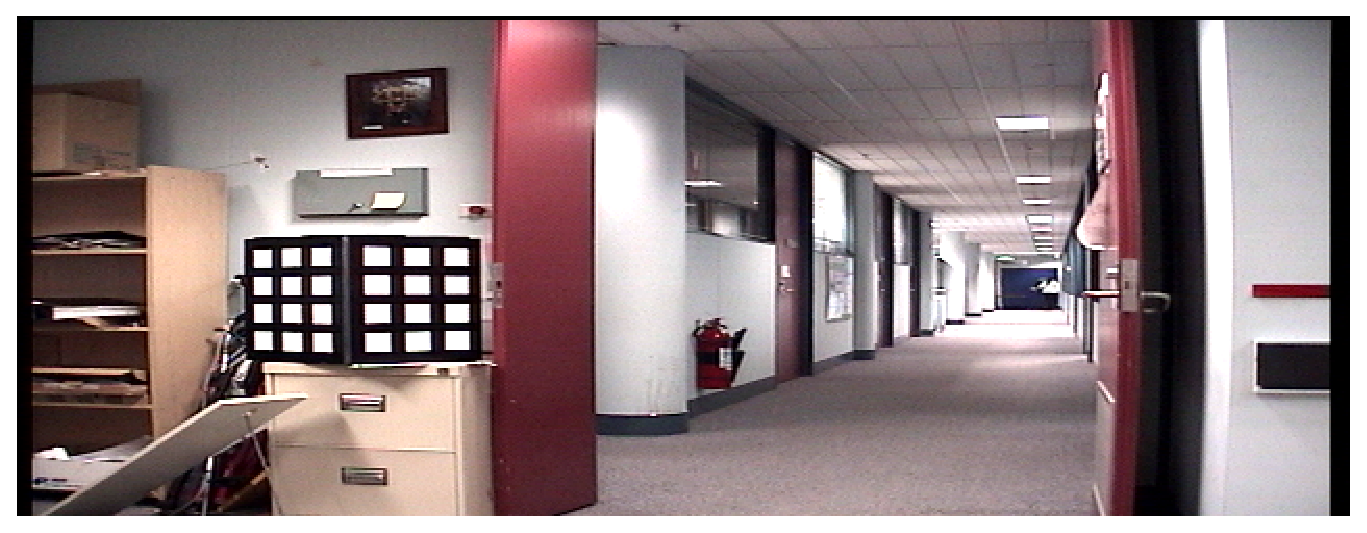
\includegraphics[width=12cm]{Pics/barrel_distortion}
}\\
\subfigure[Corrected image.]{
  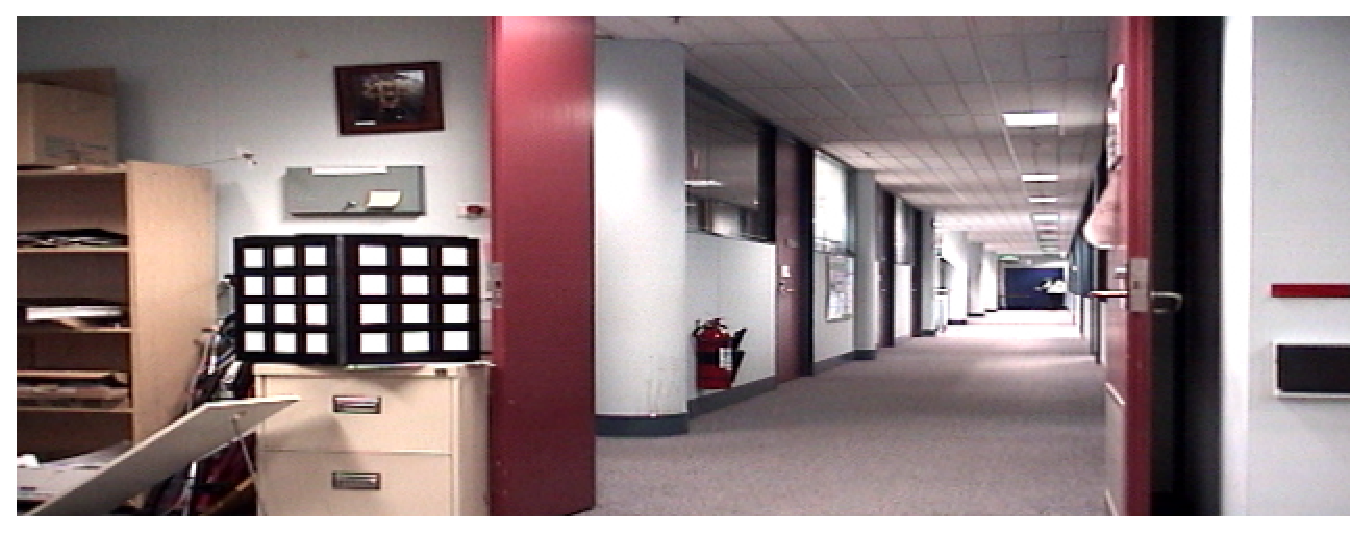
\includegraphics[width=12cm]{Pics/undist_barrel_distortion}
}

  \caption[Barrel distortion]{Effect of barrel distortion (above), and corrected image (below).}
  \label{fig:barrel_distortion}
\end{figure}

The cameras used in this experiment have a noticeable barrel
distortion, that is corrected in software. The correction is applied
off-line. \refFigure{fig:barrel_distortion} shows an example of an
original and corrected images.


\section{Feature Detector: Vertical Edges}

Vertical edges are common in human built environments. Edge detection
is a relatively fast and reliable operation. Edges are unlikely to
appear on moving objects like humans. A matched pair of edges in two
images corresponds to a line in world coordinates. A matched pair
of two vertical edges corresponds to a vertical line in world
coordinate, if the cameras a parallel to the ground plane. A vertical
line in a three dimensional space has only two degrees of freedom and
can be defined completely by a point of intersection with the ground
plane. Similarly a vertical line in an image plane can be defined
completely by a single parameter: it's distance from the left side of
an image. A camera detecting vertical edges is effectively a planar
bearing only sensor. 
%\NOTE{i.e. working in a plane only, is it a right word?}

By reducing the dimensionality of the sensor the observation model is
simplified. Which in turn makes modelling of uncertainty much more
straightforward. Since the robot motion is restricted to the plane, the
dimension corresponding to up and down can be safely ignored.

The most problematic part of the bearing only SLAM is landmark
creation. One needs at least two bearing observations from different
locations to compute an estimate of the landmark location. There are a
number of techniques commonly used \cite{bearing_only_slam}. Since the
robot in this experiment has two cameras, the problem of creating a
new landmark is simplified significantly. Having two cameras also
assists in the data association process. 

%All this makes a vertical edge a desirable candidate for
%a landmark.


%They are easy
%to extract from the image, fast and reliably. Unlikely to appear on
%moving objects (like humans), unlike features like SIFT. Generally not
%very dense (too many features can be a problem - data association,
%computation time). Can be used as bearing only observations. Easy to
%model uncertainty.  Simple update equations. Two cameras allow for
%straightforward landmark genesis, also makes data association more
%reliable.


{\bf Algorithm }\\
Run vertical edge detector on the left image. We use vertical Sobel
\cite{Hartley2004}. Only need to run it on a section of the left
image. This section is predefined at the start of the experiment and
is computed from the geometry of the stereo pair and a valid sensor
range. We are only interested in features that are reasonably
close to the camera (we use a 30 meter threshold). We can therefore
discard the extreme left part of the left image, since the features
present there won't be visible in the right image, unless they are too
far away.

Prune edges: discard short edges, also discard cluttered edges. For
all remaining edges try to find a match in the right image. Normalised
cross-correlation is used to find matches. The algorithm only needs to
search in a portion of the right image (defined by the valid sensor
range). The cameras were aligned to be close to parallel, so that
epipolar lines are roughly parallel to the $x$ axis. In the general
case the search should be performed along the epipolar line defined by
the location of the lowest pixel of the edge. Only matches with high
enough correlation are accepted. If there are to many possibilities
($> 5$) , discard the edge. If there are none, discard the
edge. Otherwise, keep best 3 matches.

We would like to avoid situations when two edges in the left image
match to the same edge in the right image. It is clearly impossible
that two distinct features in the left image appear in the same spot
in the right image, without one being hidden by another, in which case
the true location of any of features can not determined. A feature
is defined as a pair of edges; one in the left image and a matching one
in the right image. If two features share a common edge in either of
the images, they are considered to be mutually exclusive.  Given a set
of features, some of which might be mutually exclusive, we would like
to find a most likely set of compatible features.

One can visualise this problem as a graph: every pair of edges defines
a node in the graph, every two nodes of the graph are connected,
except for those nodes that share a common edge in either of the
images. The largest fully connected subgraph of this graph (commonly
referred as ``clique'' or ``maximal clique'' of a graph) corresponds
to the largest set of compatible edge pairs. A problem of finding the
clique of a graph is NP complete, meaning that for a large set of
features the solution will take forever to compute.

In our case it probably shouldn't take too long to find a true
solution by a brute force approach ($N<20$)\NOTE{what is the cost of
brute force?}. However we prefer to take a computationally faster
route to solving the problem. The approach used has $O(N^2)$
computational complexity, $N$ is a number of features being
considered. It is a greedy approach, that is choices are made in
favour of short-term gains, rather than overall return.  While it is
not guaranteed to find the best set of features, it works most of the
time. It gives much better results than just a nearest neighbour
search. \NOTE{how is this assessed}

The approach is straightforward. Sort the input set of features, most
likely features first\NOTE{define whta ''most likely'' is}. The output
set is initially empty. Take one feature from the input set, check if
it is compatible with all the features in the output set, if it is,
add it to the output set, otherwise discard it.  Keep taking features
from the input set, until none are left. This will require at most
$\frac{N(N-1)}{2}$ comparisons for a naive implementation.  Sorting
can be performed in $O(N\log N)$, therefore total computational
complexity for a naive implementation is $O(N^2)$. The compatibility
check can actually be performed at constant time. Therefor smart
implementation will have a computational complexity of $O(N\log N)$.


\begin{figure}[htbp]
  \centering
  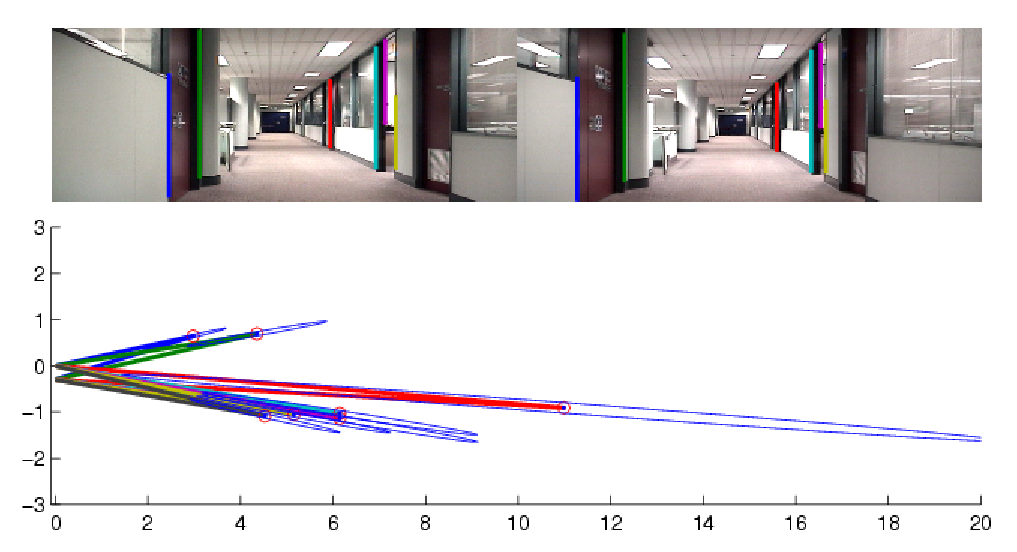
\includegraphics[width=13cm]{Pics/example_edge_detector}
  \caption{Edge Detector Output}
  \label{fig:example_edge_detector}
\end{figure}

\refFigure{fig:example_edge_detector} shows some examples of
the vertical edge feature detector working. The edge correspondences
are indicated by colour, a blue edge in the left corresponds to a blue
edge in the right image, green to green, and so forth. Locations of
the features in the reference frame of the left camera are also shown.

The appearance of a feature can provide important information to
the mapping module: it can assist in data association, especially in
situations when two edges are very close spatially (like the cyan and
magenta edges (edges 4 and 5, counting from the left) in the
\refFigure{fig:example_edge_detector})

Since vertical edges are generally uniform along the vertical
dimension, i.e. every row looks a lot like any other, edge template
can be ``compressed'' by computing the average intensity along the
vertical dimension. It is simply an average of the columns around the
edge. We use a width of 7 pixels, 3 colours per pixel, giving us 21
integer values. Using only 7 pixels per feature (21 values) greatly
reduces computational effort for template matching.  Templates are
also normalised to have zero mean, making correlation computation
really fast (21 multiplications and 20 additions, in this
case). Normalisation also makes template matching less sensitive to
variations in the lightning conditions.

\subsection{Sensor Uncertainty}

There are several sources for uncertainty in the sensor. Some
uncertainty comes from the fact that camera calibration is not
perfect. The cameras focal length $F$ and centre point $C$ are not
known exactly and might also vary slightly during the experiment. A
second source of uncertainty is the feature extraction mechanism. As
point of view changes, the edge might be picked up from a slightly
different part of the landmark. Pixel error in the right image is even
more, because the correlation search adds more uncertainty to it.
Discretisation errors add some noise as well.

Bearing is computed from the column pixel $p$ using the following equation

$$
z = f([p,C,F]^T) = \frac{p - C}{F}
$$

The Jacobian of $f$ with respect to $[p,C,F]^T$ ,$\bigtriangledown f$ is used to compute the
approximate Gaussian uncertainty of $z$ from the uncertainties of
$[p,C,F]^T$.

$$
\bigtriangledown f = \left[ 
\frac{1}{F},
\frac{1}{-F},
\frac{-p + C}{F^2}
\right]
$$

The uncertainty of the bearing can then be computed

$$
\sigma^2_z = \bigtriangledown f \left[ \begin{array}{ccc}
      \sigma^2_p & & \\
   &  \sigma^2_C & \\
  & & \sigma^2_F 
\end{array} \right] \bigtriangledown f^T.
$$



\section{Edge Landmark}

An edge landmark is basically a point landmark with some extra
attributes. The extra attributes include the normalised edge template
(7 pixel x 3 colours = 21 bytes) and a list of all observations of the
landmark.  Normalised average template is used to aid in data
association and also during the map matching when closing loops. A
list of observations is also used during data association if the
result of matching with the average template failed to produce a
definite answer (not quite the same, but not very dissimilar either).

The data structure used to hold the list of observations allows itself
to be copied in constant time, so there is no computational burden for
keeping this information. Memory requirements however grow as more
observations are collected. It is not absolutely necessary to keep all
this information, as the average template is usually sufficient. The
main motivation for keeping all observations of the landmark is to
allow accurate template matching in situations when the appearance of
the landmark changes significantly depending on the observation angle.

The goal of keeping templates is to provide a comprehensive
representation of the appearance of the landmark from various view
points. This can be achieved with relatively few templates. It is not
necessary to store all of them. \NOTE{cite Principal Component
Analysis?} This problem is however beyond the scope of this thesis.

The landmark true state ${\bf x} = \left[x,y \right]^T$ represents its
location in the local reference frame. The camera pose in the local frame
is denoted $x_c,y_c$ and camera orientation is $\theta_c$. For clarity
lets also define $x'=x-x_c$ and $y'=y-y_c$.  Observation $z_k$, and
landmark states are related by the non-linear function $h$, defined in
the equation below ($v = N(0,\sigma_{v}^2)$ is a measurement noise)

$$
z_k = h({\bf x},v) =
\frac{-x'\sin \theta_c + y' \cos \theta_c }
     {+x'\cos \theta_c + y' \sin \theta_c } + v.
$$

The true state of the landmark is not known, the estimate of the
landmark state at time $k$, $\hat{\bf x}_k$ is available
instead. The estimate error covariance for the landmark is maintained by
the EKF and is denoted $P_k$. For clarity lets also define
$\hat{x_k}'=\hat{x_k}-x_c$ and $\hat{y_k}'=\hat{y_k}-y_c$.

Let us now define a Jacobian of partial derivatives of $h$ with
respect to the landmark state

$$
H_{[i,j]} = \frac{\partial h_{[i]}}{\partial {\bf x}_{[j]}}
             \left(\hat{\bf x}_k , 0 \right).
$$

It is equal to

$$
  H = \left[ 
\begin{array}{c}
\frac{-\hat{y_k}'}
{\hat{x_k}'^2 \cos^2 \theta_c + 2\hat{x_k}'\hat{y_k}'\cos\theta_c\sin\theta_c + \hat{y_k}'^2\sin^2  \theta_c }\\
{}\\
\frac{\hat{x_k}'}
{\hat{x_k}'^2 \cos^2 \theta_c + 2\hat{x_k}'\hat{y_k}'\cos\theta_c\sin\theta_c + \hat{y_k}'^2\sin^2 \theta_c }
\end{array}
      \right].
$$

These Jacobians are used by the EKF, and also during data association,
to project landmark uncertainty into the observation space.

The Jacobian of partial derivatives of $h$ with respect
to noise is also needed by EKF, in this case it is trivial

$$
V_{[i,j]} = \frac{\partial h_{[i]}}{\partial v_{[j]}}
             \left(\hat{\bf x}_k , 0 \right) = 1.
$$


\subsection{Data Association}

First, all landmarks are projected into the observation space,both
into the left and right camera. Those landmarks that fall outside the
sensor range are discarded. For each observation the most likely
landmark is found using the nearest neighbour search. 

The quality of a match between a landmark and a single bearing
observation is computed using the following

$$
  {\bf w}_k = \int p(z_k|^z{\bf x}_k)p(^z{\bf x}_k) d^z{\bf x}.
$$

Here $^z{\bf x}_k$ is a landmark projected into the camera plane,
$p(^z{\bf x_k})$ is approximated to be a Gaussian, EKF style

$$
p(^z{\bf x}_k) = N(h(\hat{\bf x}_k,0), H P_k H^T).
$$

The term $p(z_k|^z{\bf x}_k)$ represents the measurement uncertainty,
and is also a Gaussian distribution $N(z_k ,\sigma^2_{vk})$. Since
both distributions are Gaussians, the likelihood of the match can be
computed analytically.

Both left and right bearing have to match the landmark. Total quality
of the match is a product of the left and right weights ${\bf
w}^l_k{\bf w}^r _k$.

Template matching is used to aid data association as a binary pass or
fail operator. Template matching is only performed if the spatial
tests have passed.

Nearest neighbour is not the best approach to data association. The
fact that observations were extracted from the same video frame
contains an important piece of information, it means that these
observations came from different physical entities. Nearest neighbour
search discards this information. Observations from the same video
frame can be assigned to the same landmark.

Ideally the data association process should take all available
information into consideration. One can use the joint compatibility
data association \cite{neira01:_data_assoc_stoch_mappin_using}. Or one
might explore the complete set of possible data associations directly,
by sampling from the set of all possible data association decisions
\cite{nieto2003}. In this work nearest neighbour search assisted by
template matching proved to be sufficient. However a better data
association approach is likely to improve the success rate of the
existing approach.


\subsection{Observation Update}

An observation is treated as two independent bearing only
observations. First left, then right one. The standard EKF update
equations are applied to update the estimate of the landmark
state. $P_k$ is an uncertainty of the state estimate.  Superscript
$^+$ indicates an updated estimate.

\begin{eqnarray}
K &=& P_kH(HP_kH^T + \sigma^2_{vk})^{-1}\\
\hat{\bf x}^+_k &=& \hat{\bf x}_k + 
                      K\left(z_k - h(\hat{\bf x}_k,0) \right)\\
P^+_k &=& (I - KH)P_k
\end{eqnarray}

\NOTE{Normalise EKF notation accross the whole document.}

The landmark template is also updated. It is simply an average of all
observation templates. Each landmark maintains a count of the number
of times it has been observed and a sum of all templates. The average
template is computed from the sum by simply dividing by the total
number of observations, after that the template is normalised, such
that the mean is equal to zero, and the sum of deviations from the
mean squared is equal to 1. The normalisation is needed to make the
normalised cross correlation computation faster. \NOTE{move
explanation up.}



\subsection{Genesis}

When an edge pair does not match any of the existing landmarks in
the map, a new landmark is added to the map. The initial landmark pose
and the corresponding uncertainties are computed from the observations
using the equations described below.

Let $x_r,y_r$ be the location of the right camera with respect to the
left one, and $\theta_r$ be the orientation of the right camera
relative to the left one. Let $u_l,u_r$ be the bearing observation
(tangent of the angle) from the left and right cameras
respectively. We then define the observation to be

$$
{\bf z} =  \left[
    \begin{array}{c}
       u_l\\u_r\\x_r\\y_r\\\theta_r
    \end{array}
\right].
$$

The landmark state can be computed from the observation using the
following

$$
{\bf x} = f\left({\bf z}\right) 
= \left[\begin{array}{c}
\frac{y_r - x_r\tan(\tan^{-1} u_r+\theta_r)}{u_l-\tan(\tan^{-1} u_r+\theta_r) }\\
{}\\
\frac{y_r - x_r\tan(\tan^{-1} u_r+\theta_r)}{u_l-\tan(\tan^{-1} u_r+\theta_r)}u_l
\end{array}
\right].
$$

We assume that the uncertainty of the observation is a Gaussian with
the following block-diagonal covariance matrix

$$
C_z = \left[
  \begin{array}{ccc}
    \sigma^2_{ul} &             & \\
                & \sigma^2_{ur} & \\
                &             & \Sigma_{xy\theta}
  \end{array}
\right].
$$

We then compute the Jacobian of $f$ with respect to each of the
observation elements

$$
{\bf J}_{[i,j]} = \frac{\partial f_{[i]}}
{\partial z_{[j]}}\left(z \right).
$$

The initial uncertainty of the feature is then set to

$$
P = {\bf J} C_z {\bf J}^T.
$$

The landmark template is set to that of the observation.

\section{Defining Map Region}

Unlike laser range sensors, vision sensors can not provide free space
information easily. While it is not impossible to extract free space
information from a sequence of images, it is definitely not
trivial. It is therefore assumed that no free space information is
available. The approach for defining region bundaries was identical to
that used for the Victoria park data set, with an excpetion of the
size of the initial region and the size of grid cells, which wer set
to be smaller.

\section{Results}

Vision data has been collected together with the laser corner data, so
a comparison can be made between vision and laser experiments. The vision
data set was processed with 100 and 300 particles. One hundred runs of
the algorithm were taken to judge the robustness of the algorithm (100
for 100 particles and 100 for 300 particles).
%\subsection{Maps}

Figures~\ref{fig:edge_map_300p} and \ref{fig:edge_map_100p} show the
map produced for one of the runs using 300 and 100 particles
respectively. Local maps are projected into the reference frame of the
first region. 

Vision is a much more challenging sensor than laser. While most of the
runs have produced good map, many runs
failed. Table~\ref{tab:results_vision} lists the success/failure rates
for the experiment.

\begin{table}[ht]
\center
\begin{tabular}{r|c|c|c}
Num. Particles & Consistent & Consistent but improper & Inconsistent\\
\hline
100 & 67 & 1 & 32\\
300 & 71 & 5 & 24\\
\end{tabular}
\caption{Summary of the experiments.}
\label{tab:results_vision}
\end{table}

Increasing the number of particles makes the algorithm more robust,
but only slightly. Figures~\ref{fig:edge_map_300p_broken} and
\ref{fig:edge_map_300p_borken2} show examples when HTSLAM did not
succeed to build a proper map. \refFigure{fig:edge_odo_all} shows the
paths of all 100 experiments projected into the reference frame of the
first region.

%Refer to the laser results, same data set. 

\begin{figure}[htbp]
  \centering

  \subfigure[Projection of the HTSLAM map in the reference frame of map 1.]{
    \includegraphics[width=15cm]{Pics/edge_map_300p}
  }\\
  \subfigure[Topological path of the robot.]{
    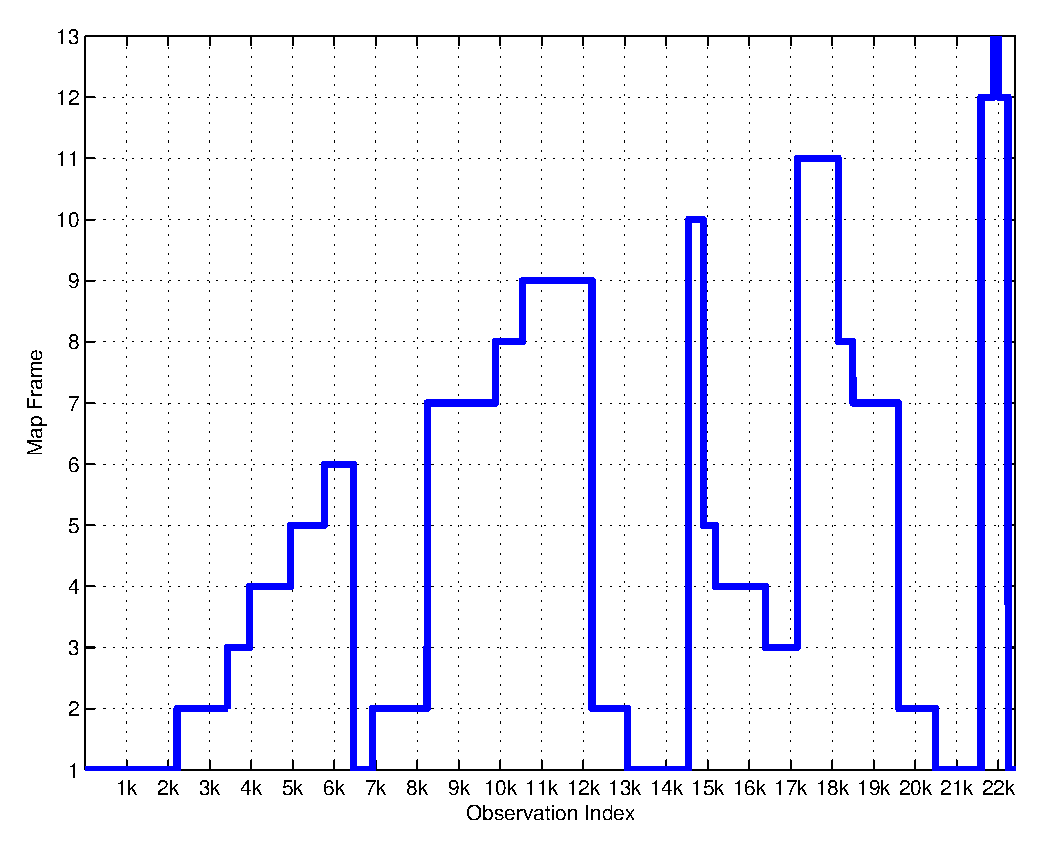
\includegraphics[width=10cm]{Pics/edge_odo_300p}
  }

  \caption{Map of edges (300 particles/map 52)}
  \label{fig:edge_map_300p}
\end{figure}

\begin{figure}[htbp]
  \centering
  \subfigure[Projection of the HTSLAM map in the reference frame of map 1.]{
    \includegraphics[width=15cm]{Pics/edge_map_100p}
  }
  \subfigure[Topological path of the robot.]{
    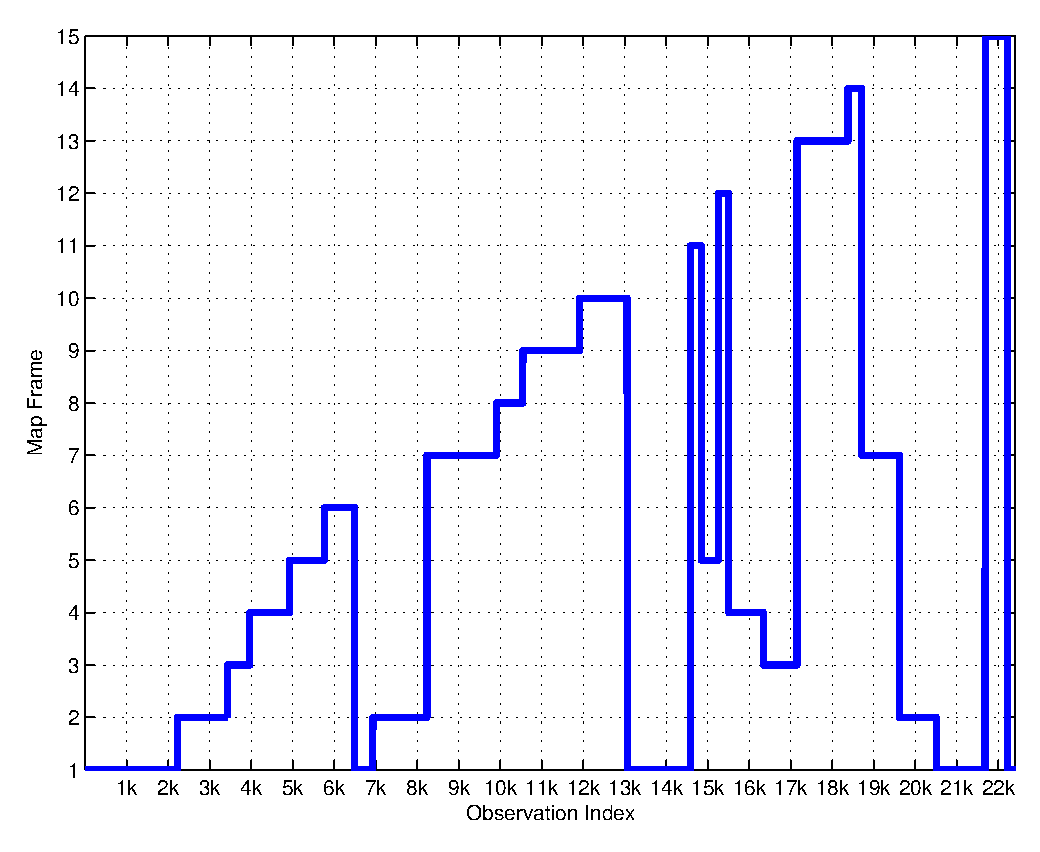
\includegraphics[width=10cm]{Pics/edge_odo_100p}
  }
  \caption{Map of edges (100 particles/map 89)}
  \label{fig:edge_map_100p}
\end{figure}

\begin{figure}[htbp]
  \centering
  \subfigure[Projection of the HTSLAM map in the reference frame of map 1.]{
    \includegraphics[width=15cm]{Pics/edge_map_300p_broken}
  }
  \subfigure[Topological path of the robot.]{
    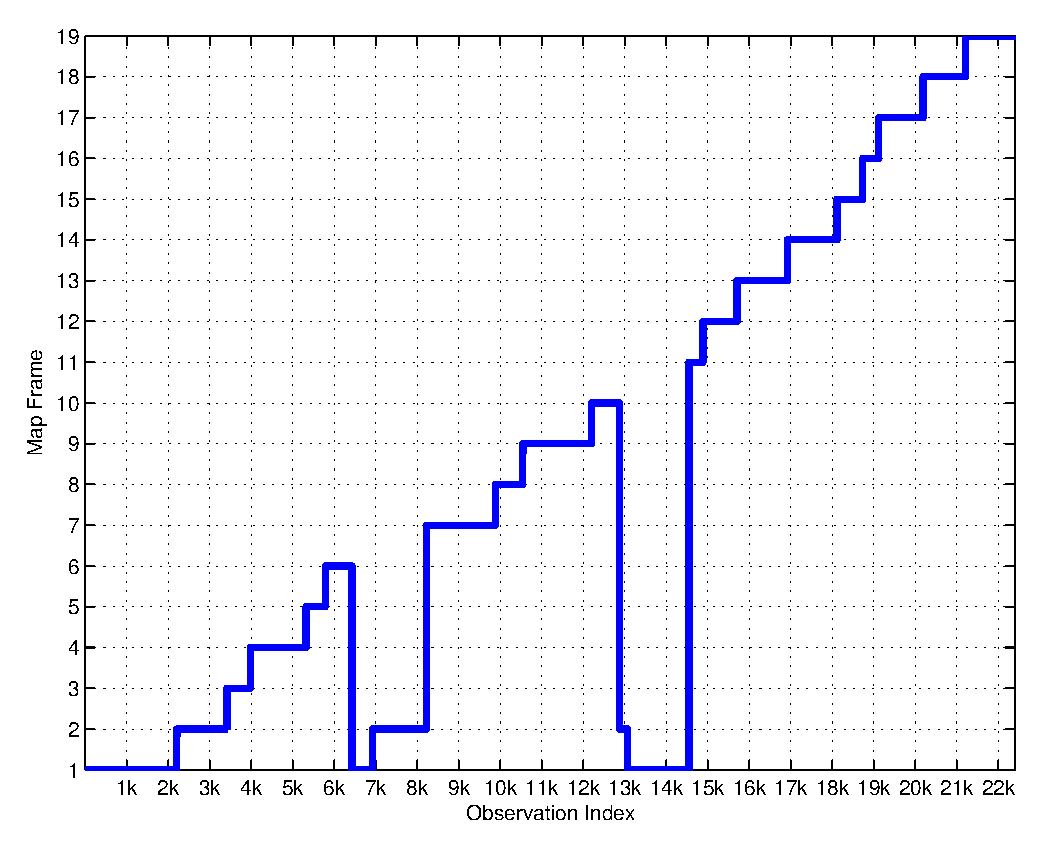
\includegraphics[width=10cm]{Pics/edge_odo_300p_broken}
  }
  \caption{Jumped out, failed to come back(300 particles/map 40).  Topologically correct, but not ``optimal''}
  \label{fig:edge_map_300p_broken}
\end{figure}

\begin{figure}[htbp]
  \centering
  \subfigure[Projection of the HTSLAM map in the reference frame of map 1.]{
    \includegraphics[width=15cm]{Pics/edge_map_300p_broken2}
  }
  \subfigure[Topological path of the robot.]{
    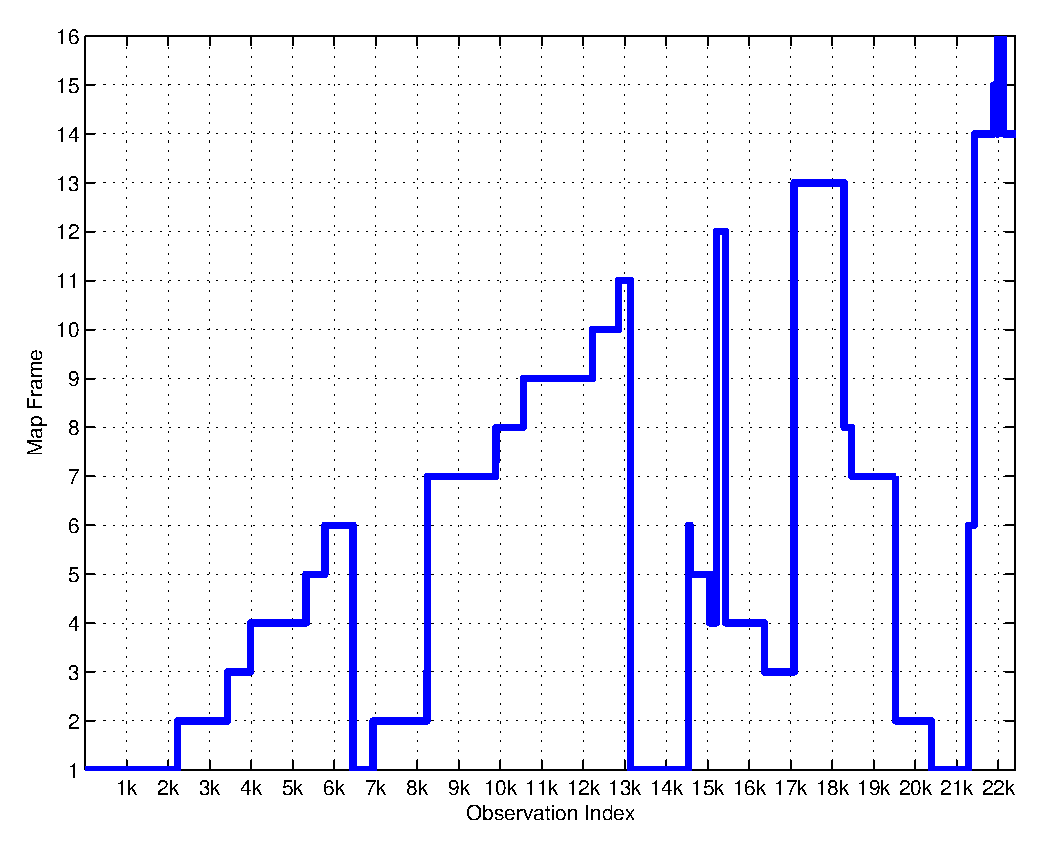
\includegraphics[width=10cm]{Pics/edge_odo_300p_broken2}
  }

  \caption{Failed transition 7 to 2 (300 particles/map
    18).}
  \label{fig:edge_map_300p_borken2}
\end{figure}

\begin{figure}[htbp]
  \centering
  \subfigure[100 particles]{
    \includegraphics[width=15cm]{Pics/edge_odo_all_100p}
  }
  \subfigure[300 particles]{
    \includegraphics[width=15cm]{Pics/edge_odo_all_300p}
  }
  \caption{Global Path over 100 test runs.}
  \label{fig:edge_odo_all}
\end{figure}



\subsection{Error Analysis}

There are a number of reasons for the poor performance of the vision
SLAM:

\begin{itemize}
\item Data association is quite challenging with this type of
sensor. 
\item Poor calibration of the sensor.
\item Unmodelled odometric bias.
\end{itemize}

Camera provides a rather accurate bearing and very uncertain range
measurement. As a result the performance of the sensor is sensitive to
calibration errors. The more accurate your sensor is, the more obvious
the impact of biases in the error model will be.

Data association is very tricky when revisiting the region, while
travelling in opposite direction from the first pass.



\SILENT{Discuss: the effect of non-optimal region assignment, the
  difficulty in observing landmark the other way (main problem is data
  association), effect number of particles has on success rates, more
  is better as expected. Take note that failure mostly occurred when
  traversing the other way, so is probably has more to do with the
  sensor than with our approach to mapping, although acknowledge that
  transition can ``trigger'' failure by spreading particles thin,
  combined with difficult sensory situation it leads to failure some
  times, mainly after map 2 to 7 transition. 

Discuss possible sources of failure. Two classes: global map, local
map. Global include: incorrect map matching, transitions to the
wrong region, failing to close the loop.

Local sources of error: unmodelled biases in the sensory or odometry
input, improperly modelled sensory noise, wrong data associations,
unmodelled dimension.
}


% LocalWords:  epipolar EKF Jacobians Gaussians IDE Sobel  cyan discretisation
% LocalWords:  HTSLAM odometric odometry
